\documentclass{article}

\usepackage[UTF8]{ctex}
\usepackage{amsmath}
%\usepackage{steinmetz}
\usepackage{graphicx}
\usepackage{geometry}
\geometry{a4paper,scale=0.75}
% left=2cm,right=2cm,top=1cm,bottom=1cm
\title{目标检测Notebook}
\author{叶亮}
\date{\today}
\begin{document} 
\maketitle
\section{Loss}
\subsection{IoU loss}


\subsection{GIoU loss}

\subsection{DIoU loss}

Code optimization, the calculation of distance between two center points of bboxes.
\begin{equation}
\begin{aligned}
(C_1-C_2)^2)&= ((x1_{C1}+x2_{C1})/2-(x1_{C2}+x2_{C2})/2)^2 \\
&=((x1_{C1}+x2_{C1})-(x1_{C2}+x2_{C2}))^2/4 \\
\end{aligned}
\end{equation}
\subsection{CIoU loss}
\subsection{BIoU loss}

\section{Activation}
\subsection{Sigmoid}

\subsection{ReLU}

\subsection{SiLU}
Sigmoid Linear Unit
\begin{align}
\text{silu}(x) = x * \sigma(x), \text{where } \sigma(x) \text{ is the logistic sigmoid.}
\end{align}
\begin{figure}[htp]
\centering
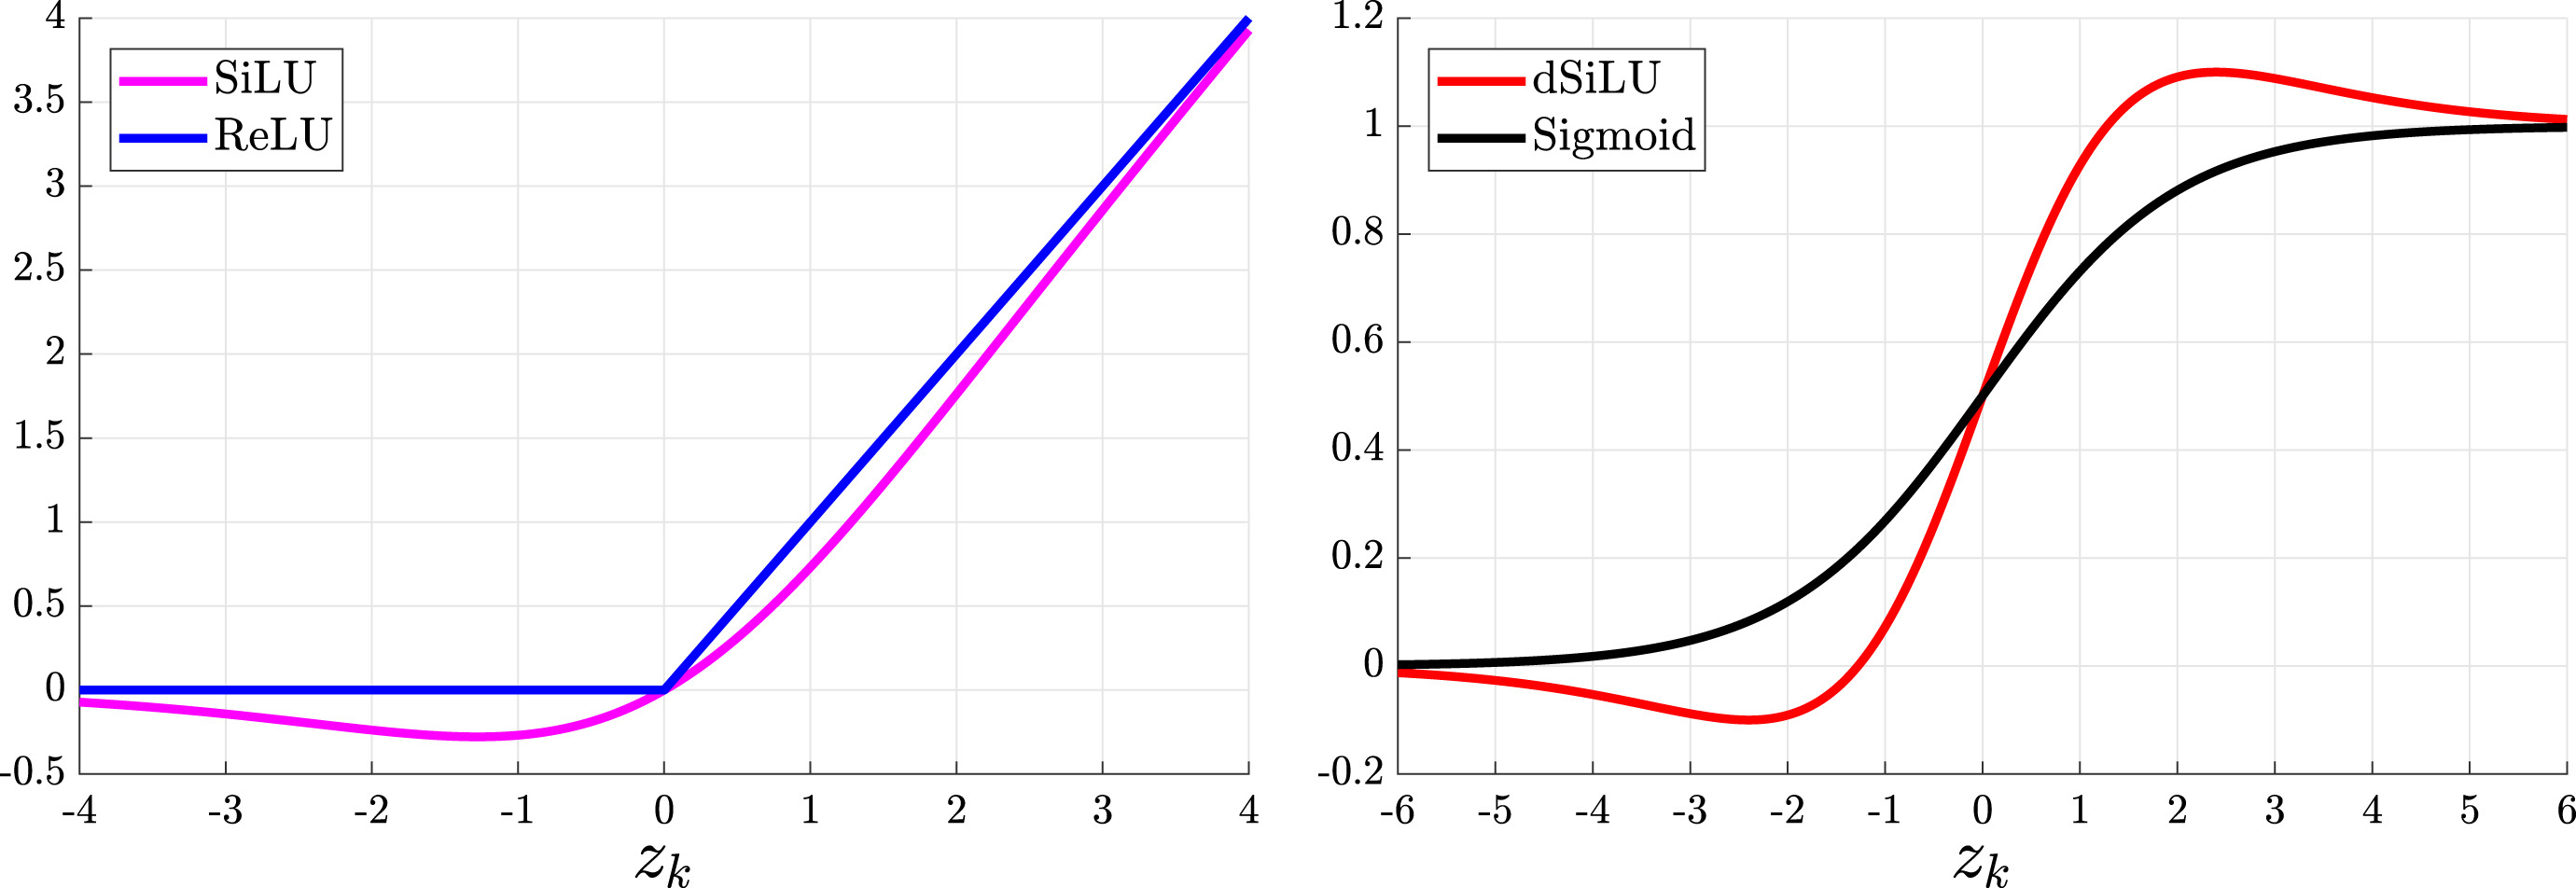
\includegraphics[scale=1]{images/SiLU.jpg}
\caption{The activation functions of the SiLU and the ReLU (left panel), and the dSiLU and the sigmoid unit (right panel)}
\label{SiLU}
\end{figure}
\section{mmdetection}

\subsection{anchor}
mmdetection中,在retinanet, R-CNN等非ssd系列检测器的grid anchor生成中,在grid中每个anchor的坐标表示为(xmin,ymin,xmax,ymax)。anchor参数包含strides, ratios, scales, base sizes等. 其中strides为特征图的步长,ratios为宽高比,scales为anchor的缩放因子。计算过程如下:

1. 根据featmap生成grid.其中grid坐标为i * featmap size for i in grid size.

2. grid中每个cell根据 ratios,  scales和base sizes计算anchors,$xmin = grid_i -  basesize*scales*ratios, xmax = grid_i +basesize*scales*ratios$.
每个anchor的形式为(xmin,ymin,xmax,ymax),且均

 具体计算方式可参考\textbf{core/anchor/anchor\_generator.py}中部分。

\subsection{coder}
在RetinaNet、SSD、Cascade R-CNN等网络中,网络预测的bbox都会进行Delta xywh编码,即将原始的(xmin, ymin, xmax, ymax)进行编码,计算相对距离,来减小回归的过拟合,提升回归的稳定性。
\begin{equation}
\begin{aligned}
&\delta_x = (g_x-p_x)/p_w	   & \delta_y = (g_y - p_y)/p_h \\
&\delta_w = \log{\frac{g_w}{p_w}}	&\delta_h = \log{\frac{g_h}{p_h}}
\end{aligned}\label{bbox_coder}
\end{equation}

上述公式计算得到的$\delta$值通常很小,因为网络通常只对p进行少量微调,导致回归loss比分类loss小很多。为了提升学习的有效性,$\delta$通常需要经过均值和方差进行标准化.

\begin{equation}
\begin{aligned}
\delta_{x}^{'}=\frac{\delta_x-\mu_x}{\rho_x}
\end{aligned}
\end{equation}

\section{training}
\subsection{Optimizer}
\subsubsection{warmup}
warmup通常有三个方式:linear, constant, exp. 通常需要设置warmup的迭代数$iter_{total}$和warmup的增加比率ratio,
\begin{align}
lr_t = lr_{constant}*ratio
\end{align}
\begin{equation}
\begin{aligned}
lr_t = lr_{const}*(1-k), \\
k= (1-iter_t /iter_{total}) * (1-ratio)
\end{aligned}
\end{equation}
\begin{align}
lr_t = lr_{const}*k, \\
k=ratio^{1-iter_t/iter_{total}}
\end{align}

\section{Yolov4}
Yolov4的实现过程中,anchor的生成以及label与anchor的对应关系的构建方法。
\subsection{Anchor generation \& target build}
与retinanet,rcnn系列等bbox预测不同的是,yolo模型推理得到的结果(x,y,w,h)需要经过如下公式进行编码:
\begin{equation}
\begin{aligned}
b_x = \sigma(t_x)+c_x \\
b_y = \sigma(t_y)+c_y \\
b_w = p_we^{t_w} \\
b_h = p_he^{t_h}
\end{aligned}
\end{equation}
\begin{figure}[htp!]
\centering
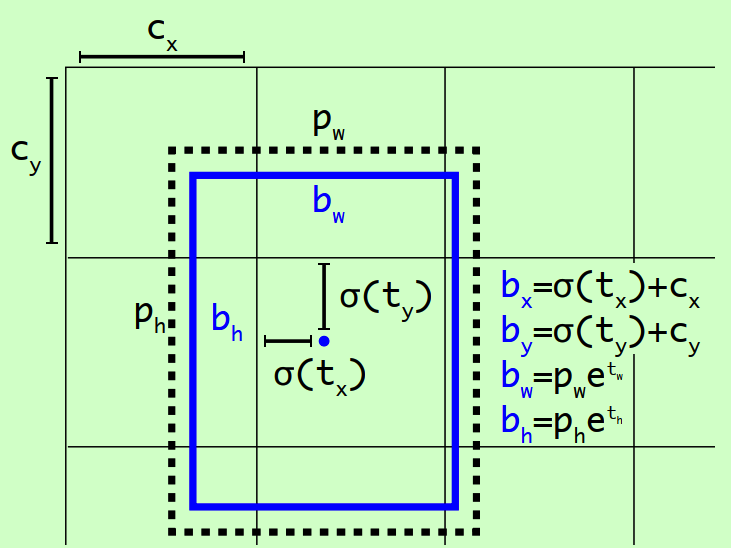
\includegraphics[scale=0.3]{images/yolo_bbox.png}
\caption{Yolo bbox prediction}
\end{figure}

\section{Yolov5}
\subsection{Model}
Focus结构: Focus模块中,首先将一幅图,按照隔点采样(::2,1::2)的方式,将一个图片分成四幅图,然后将这四幅图拼接到一块,形成$3*4=12$通道的特征图,再做卷积操作,这样来实现下采样和卷积操作。

\section{backbone}
\subsection{Regularization}
\subsubsection{Dropout}
原理,dropout随机丢弃神经元(全连接中输入神经元),实现方式为$keep_prob$,每个神经元生成一个随机数$k,k<keep_prob$即丢弃。优点,该方法有利于分类中泛化能力的提升.
\subsubsection{Drop Connect}
\subsubsection{Drop block}


\section{Refinedet}
\subsection{Anchor}
Refine中的anchor计算。对于每一个feature map, 首先计算其mesh grid,然后计算每个框的中心点$(x,y)=(\frac{i+0.5}{feat\_size},\frac{j+0.5}{feat\_size})$,然后根据每个feature map对应的anchor box的大小,计算anchor的长和宽$WH_{ki}=\frac{box_k}{image\_size}$, k表示第k层特征图,i表示第i个网格. e.g, 使用四个feature level, $box=[32,64,128,256], image\_size=320, feat\_size=[40,20,10,5], aspect\_ ratio=[2,2,2,2]$, 那么最终生成$40*40*3+20*20*3+10*10*3+5*5*3=6375$个anchor.

\subsection{Loss}
计算过程分为arm和odm,其中arm预测分别输出$num\_anchor*4$和$num\_anchor*2$通道的特征图(坐标,是否包含目标);odm预测分别输出$num\_anchor*4$和$num\_anchor*num\_classes$通道的特征图(坐标,类别数量)。每层特征图的目标数量则为$N_i*H_i*num\_anchor$。

在loss计算过程中,分别计算分类loss和回归loss.其中分类使用交叉熵,回归使用smooth l1



\section{Dataset}
\subsection{COCO Dataset}
COCO dataset 全称 Common Objects in Context. 共有80个类。共有三种标注类型:object instance, object keypoints, image captions。使用json文件进行存储。
\subsubsection{object instance}
{
    "info": info,
    "licenses": [license],
    "images": [image],
    "annotations": [annotation],
    "categories": [category]
}

\section{Detector}
\subsection{CornerNet, CenterNet}
\subsubsection{targets computation}
在anchor free网络中,生成gt bbox的heatmap target时,相应的高斯半径的计算方式如下。一共存在三种情况:
1,生成的target与gt bbox有重叠部分,其中一个corner在gt box内部,另一个在gt box外部。
\begin{gather}
        \cfrac{(w-r)*(h-r)}{w*h+(w+h)r-r^2} \ge {iou} \quad\Rightarrow\quad
        {r^2-(w+h)r+\cfrac{1-iou}{1+iou}*w*h} \ge 0 \\
        {a} = 1,\quad{b} = {-(w+h)},\quad{c} = {\cfrac{1-iou}{1+iou}*w*h} \\
        {r} \le \cfrac{-b-\sqrt{b^2-4*a*c}}{2*a}
\end{gather}
2.两个corner都在gt box里面
\begin{gather}
\cfrac{(w-2*r)*(h-2*r)}{w*h} \ge {iou} \quad\Rightarrow\quad
        {4r^2-2(w+h)r+(1-iou)*w*h} \ge 0 \\
        {a} = 4,\quad {b} = {-2(w+h)},\quad {c} = {(1-iou)*w*h} \\
        {r} \le \cfrac{-b-\sqrt{b^2-4*a*c}}{2*a}
\end{gather}
3.两个corner都在gt box外部
\begin{gather}
\cfrac{w*h}{(w+2*r)*(h+2*r)} \ge {iou} \quad\Rightarrow\quad
        {4*iou*r^2+2*iou*(w+h)r+(iou-1)*w*h} \le 0 \\
        {a} = {4*iou},\quad {b} = {2*iou*(w+h)},\quad {c} = {(iou-1)*w*h} \\
        {r} \le \cfrac{-b+\sqrt{b^2-4*a*c}}{2*a}
\end{gather}
高斯核的计算
\begin{align}
\exp^{\cfrac{-(x*x+y*y)}{2*\sigma*\sigma}}
\end{align}

\subsubsection{decode heatmap}
对heatmap进行解码,遵循如下顺序:1. nms on heatmap. 2. get topk positions from heatmap. 3. decode offset and wh size.

\section{Optical Character Recognition}
\subsection{DBNet}
Real-Time Scene Text Detection with Differentiable Binarization\cite{liao2020real}.
\subsubsection{Related work}
最近的OCR可分为两种:Regression-based and segmentation-based.

\textbf{Regression-based methods} 直接回归文本实例的坐标框,使用NMS后处理。大部分模型达不到精准的文本框检测(非矩形,非旋转矩形等),尤其是弯曲的文本位置。

\textbf{Segmentation-based methods} 结合Pixel-level prediction and post-processing 来获取文本位置。
\begin{figure}[htp!]
\centering
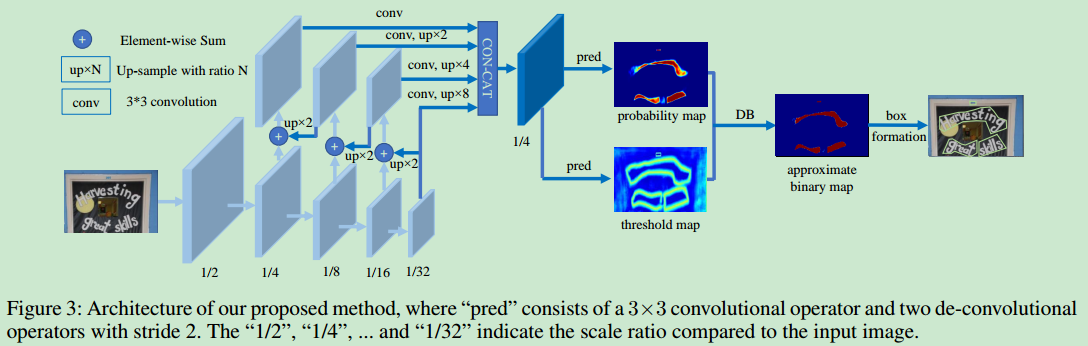
\includegraphics[scale=0.4]{images/dbnet.png}
\caption{Architecture of the DB-Net}
\label{Fig.dbnet}
\end{figure}

\subsubsection{Methodology}
如图Fig. \ref{Fig.dbnet}所示,使用FPN作为backbone,在1/4阶段做预测,生成概率图($P$)和阈值图($T$),并通过P和T来计算approximate binary map($\hat{B}$).二值化过程可表述为如下公式:
\begin{equation}
B_{i,j} = \left\{
\begin{array}{lr}
1 & if \: P_{i,j} >=t, \\
0 & otherwise.
\end{array}
\right.
\label{Eq.binarization}
\end{equation}
\textbf{Differentiable binarization} 公式\ref{Eq.binarization}不可微。所以在训练时不能通过网络对其进行优化,因此论文提出如下近似step function:
\begin{align}
\hat{B}_{i,j}=\dfrac{1}{1+e^{-k(P_{i,j}-T_{i,j})}}
\end{align}
其中,$k$表示增强因子,设置成50.DB提升性能可归结于梯度方向传播。以二值交叉熵为例,定义$f(x)=\dfrac{1}{1+e^{-kx}}$为DB函数,其中$x=P_{i,j}-T_{i,j}$,正类标签的loss $l_+$和负类标签的loss $l_-$分别为:
\begin{equation}
\begin{aligned}
l_+ = -\log{\dfrac{1}{1+e^{-kx}}} \\
l_- = -\log{(1-\dfrac{1}{1+e^{-kx}})}
\end{aligned}
\end{equation}
使用链式规则可以得到如下微分:
\begin{align}
\dfrac{\partial l_+}{\partial x} = -kf(x)e^{-kx} \\
\dfrac{\partial l_x}{\partial x} = kf(x)
\end{align}

\textbf{Label Generation}
PSENet生成方法:给定文本图像,每个文本区域的多边形由一系列线段进行描述:
\begin{align}
G = \{ S_k \}_{k=1}^n
\end{align}
其中,$n$表示顶点数量,在不同的数据集中不一样。ICDAR 2015为4,CTW1500为16.然后使用Vatti clipping算法将多边形$G$收缩程$G_s$得到正类区域.其中,收缩的偏移量D由原多边形的周长L和面积A计算得到:
\begin{align}
D=\dfrac{A(1-r^2)}{L}
\end{align}
$r$为收缩比例,一般设置为0.4. 通过类似方法,为阈值图生成标签。1. 多边形$G$通过相同的偏移$D$进行膨胀得到$G_d$.2. 将$G_s$和$G_d$之间的间隙(gap)作为文本区域的边界,其中阈值图的标签通过计算距离$G$中最近的线段距离得到。

\textbf{Optimization}

Loss表示为概率图$L_s$, 二值图$ L_b $和阈值图$L_t$的加权和:
\begin{align}
L=L_s + \alpha \times L_b + \beta \times L_t
\end{align}
$\alpha$和$\beta$分别设置为1.0和10。对$L_s$和$L_b$应用binary cross-entropy(BCE)loss,使用hard negative mining来缓解正负样本的非平衡问题:
\begin{align}
L_s = L_b = \sum_{i \in S_l}{y_i \log{x_i} + (1 - y_i) \log{1 - x_i}} 
\end{align}
其中,$S_l$为采样集,正负样本比例为1:3.

$L_t$使用$L_1$距离和来计算loss,为膨胀后的文本多边形区域$G_d$内预测和标签的距离:
\begin{align}
L_t = \sum_{i \in R_d}{\left| y_i^* - x_i^* \right|}
\end{align}
其中,$R_d$为膨胀后的多边形$G_d$内的像素索引集合,$y_i^*$为阈值图标签

在推理阶段,可以只用概率图或近似二值图来生成文本坐标框,其结果相似,任选一即可。论文中,为了更好的效率,使用概率图来生成文本框,这样可以移除阈值图。即,box处理过程为三个步骤:1)从概率图/近似二值图通过固定阈值(0.2)来首次二值化得到二值化图; 2)从二值图得到连接区域(收缩的文本区域); 3)使用偏移量$D'$, Vatti clipping算法来膨胀收缩区域。$D'$计算方式为:
\begin{align}
D' = \dfrac{A' \times r'}{L'}
\end{align}
其中,$A'$为收缩多边形的面积;$L'$为收缩多边形的周长;$r'$通过经验设置为$1.5$.

\subsubsection{Implementation Details}
数据集介绍: \textbf{SynthText},\textbf{MLT-2017 dataset},\textbf{ICDAR 2015 dataset},\textbf{MSRA-TD500 dataset},\textbf{CTW1500 dataset},\textbf{Total-Text dataset}.

训练时,使用SynthText预训练100k iteration, 然后在真实样本上微调1200epochs。batch size 16,使用余弦学习率下降策略。其中当前迭代的学习率为$lr_{init} \times (1 - \dfrac{iter}{max\_iter})^{power}$.初始学习率为$0.007$,$power$为0.9.weight decay of 0.0001, momentum of 0.9.

数据增强:1)随机旋转,角度区间$(-10^\circ,10^\circ)$;2)随机裁剪;3)随机翻转。所有处理图片均resize到640x640。

\bibliographystyle{IEEEtran}
\bibliography{reference.bib}


\end{document}